The work presented here contributes to a compositional theory of
``co-design'' that allows to optimally design a robotic platform.
In this framework, a user models each subsystem as a monotone relation
between \F{functionality provided} and \R{resources required}.
These models can be easily composed to express the co-design constraints
between different subsystems. The user then queries the model, to
obtain the design with minimal resources usage, subject to a lower
bound on the provided functionality. This paper concerns the introduction
of uncertainty in the framework. Uncertainty has two roles: first,
it allows to deal with limited knowledge in the models; second, it
also can be used to generate consistent relaxations of a problem,
as the computation requirements can be lowered should the user accept
some uncertainty in the answer.


\section{Introduction}

The design of a robotic platform involves the choice and configuration
of many hardware and software subsystems (actuation, energetics, perception,
control, \dots) in an harmonious entity in which all \emph{co-design
constraints} are respected. Because robotics is a relatively young
discipline, there is still little work towards obtaining systematic
procedures to derive optimal designs. Therefore, robot design is a
lengthly design process mainly based on empirical evaluation and trial
and error. The work presented here contributes to a theory of co-design
that allows to optimally design a robotic platform based on formal
models of the performance of its subsystems. The goal is to allow
a designer to create better designs, faster. This paper describes
the introduction of uncertainty in the theory.

\begin{figure}
    \begin{centering}
        \includegraphics[scale=0.33]{unc_bigproblem}
    \end{centering}
    \caption{Monotone Co-Design Problems (MCDPs) can capture
    much of the complexity of the optimal robot design process. The user
    defines a co-design diagram by hierarchical composition and arbitrary
    interconnection of primitive ``design problems'', modeled as monotone
    relations between \F{functionality} and \R{resources}. The semantics
    of the MCDP of the figure is the minimization of the \R{total mass}
    and \R{cost} of the platform, subject to functionality constraints
        (\F{distance}, \F{payload}, \F{number of missions}). This paper
        describes how to introduce uncertainty in this framework, which allows,
        for example, to introduce parametric uncertainty in the definition
        of components properties (\eg  specific cost of batteries).}

    \label{fig:Example1}
\end{figure}


\subsubsection*{Previous work}

In previous work~\cite{censi15monotone,censi15same,censi16codesign_sep16},
I have proposed a compositional theory for co-design. The user defines
``design problems'' (DPs) that describe the constraints for each
subsystem. These DPs can then be hierarchically composed and interconnected
to obtain the class of Monotone Co-Design Problems (MCDPs).

An example of MCDP is sketched in~\cref{fig:Example1}. The
design problem consists in finding an optimal configuration of a UAV,
optimizing over actuators, sensors, processors, and batteries. Each
design problem (DP) is formalized as a relation between \F{functionality}
and \R{resources}. For example, the functionality of the UAV is parameterized
by three numbers: the \F{distance to travel} for each mission; the
\F{payload to transport}; the \F{number of missions} to fly. The
optimal design is defined as the one that satisfies the functionality
constraints while using the minimal amount of \R{resources} (\R{cost}
and \R{mass}).

The convenience of the MCDP framework is that the user can define
design problems for each subsystem and then compose them. The definition
of the DPs is specified using a domain-specific language that promotes
composition and code reuse; the formal specification is contained
in the supplementary materials. In the figure, the model is exploded
to show how actuation and energetics are modeled. Perception is modeled
as a relation between \F{the velocity of the platform} and the \R{power}
required. Actuation is modeled as a relation between \F{lift} and
\R{power}/\R{cost}. Batteries are described by a relation between
\F{capacity} and \R{mass}/\R{cost}. The interconnection between
these describe the ``co-design constraints'': \eg , actuators must
lift the batteries, the batteries must power the actuators. In this
example, there are different battery technologies (LiPo, \etc), each
specified by specific energy, specific cost, and lifetime, thus characterized
by a different relation between \F{capacity}, \F{number of missions}
and \R{mass} and \R{cost}.

Once the model is defined, it can be queried to obtain the \emph{minimal}
solution in terms of resources \textemdash{} here, \R{total cost}
and \R{total mass}. The output to the user is the Pareto front containing
all non-dominated solutions. The corresponding optimization problem
is, in general, nonconvex. Yet, with few assumptions, it is possible
to obtain a systematic solution procedure, and show that there exists
a dynamical system whose fixed point corresponding to the set of minimal
solutions.


\subsubsection*{Contribution}

This paper describes how to add a notion of \emph{uncertainty} in
the MCDP framework.
The model of uncertainty considered is interval
uncertainty on arbitrary partial orders.
For a poset~$\left\langle \posA,\posleq\right\rangle $,
these are sets of the type~$\{x\in\posA\colon a\posleq x\posleq b\}$.
I will show how one can introduce this type of uncertainty in the
MCDP framework by considering ordered pairs of design problems.
Each
pair describes lower and upper bounds for resources usage.
These \emph{uncertain
design problems} (UDPs) can be composed using series, parallel, and
feedback interconnection, just like their non-uncertain counterparts.

The user is then presented with \emph{two} Pareto fronts, corresponding
to a lower bound and an upper bound for resource consumption, in the
best case and in the worst case, respectively.

This is different from the usual formalization of ``robust optimization''~(see
\eg , \cite{bertsimas11theory,ben-tal09}), usually formulated as
a ``worst case'' analysis, in which one the uncertainty in the problem
is described by a set of possible parameters, and the optimization
problem is posed as finding the one design that is valid for all cases.

Uncertainty plays two roles: it can be used as a \emph{modeling} \emph{tool},
where the relations are uncertain because of our limited knowledge,
and it can be used as a \emph{computational} \emph{tool}, in which
we deliberately choose to consider uncertain relations as a relaxation
of the problem, to reduce the computational load, while maintaining
precise consistency guarantees. With these additions, the MCDP framework
allows to describe even richer design problems and to efficiently
solve them.


\subsubsection*{Paper organization}

%\Cref{sec:Design-Problems} and \ref{sec:Monotone-Co-Design-Problems}
%summarize previous work.

They give a formal definition of design problems
(DPs) and their composition, called Monotone Co-Design Problems (MCDPs).
\Cref{sec:UDP} through~\cref{sec:Approximation-results}
describe the notion of Uncertain Design Problem (UDP), the semantics
of their interconnection, and the general theoretical results. \cref{sec:Applications}
describes three specific applications of the theory with numerical
results. The supplementary materials include detailed models written
in MCDPL and pointers to obtain the source code and a virtual machine
for reproducing the experiments.


\section{Design Problems}

\emph{A design problem} (DP) is a monotone relation between \emph{\F{provided functionality}}
and \emph{\R{required resources}}. \F{Functionality} and \R{resources}
are complete partial orders (CPO)~\cite{davey02}, indicated by~$\langle\funsp,\posleq_{\funsp}\rangle$
and~$\langle\ressp,\posleq_{\ressp}\rangle$. The graphical representations
uses nodes for DPs and green (red) edges for \F{functionality} and
\R{resources}~(\cref{fig:dp}).

\captionsideleft{\label{fig:dp}}{\includegraphics[scale=0.33]{unc_dpcartoon}}
\begin{example}
    The first-order characterization of a battery is as a store of energy,
    in which the \F{capacity {[}kWh{]}} is the \F{functionality} (what
    the battery provides) and \R{mass} {[}kg{]} and \R{cost} {[}\${]}
    are \R{resources} (what the battery requires)~(\cref{fig:battery1}).
\end{example}
\captionsideleft{\label{fig:battery1}}{\includegraphics[scale=0.33]{unc_battery_masscost}}

\noindent In general, fixed a functionality~$\fun\in\funsp$, there
will be multiple resources in~$\ressp$ sufficient to perform the
functionality that are uncomparable with respect to~$\posleq_{\ressp}$.
For example, in the case of a battery one might consider different
battery technologies that are uncomparable in the \R{mass}/\R{cost}
resource space~(\cref{fig:multiple}).

\captionsideleft{\label{fig:multiple}}{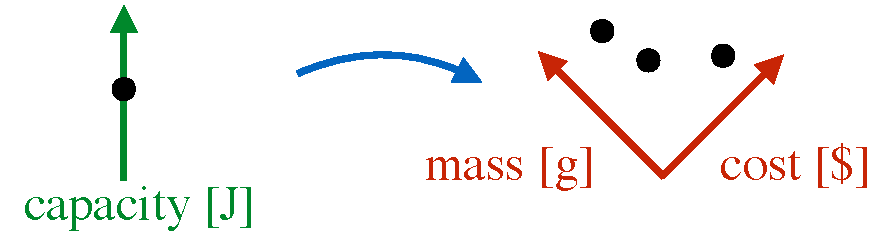
\includegraphics[scale=0.33]{reits2_battery2_h}}

A subset with ``minimal'', ``uncomparable'' elements is called
``antichain''. This is the mathematical formalization of what is
informally called a ``Pareto front''.


%\begin{definition}\label{def:antichain-paper2}
%  An \emph{antichain}~$S$ in a poset~$\left\langle \posA,\posleq\right\rangle $
%  is a subset of~$\posA$ such that no element of~$S$ dominates another
%  element: if~$x,y\in S$ and~$x\posleq y$, then~$x=y$.
%\end{definition}
%\begin{lemma}\label{lem:orderantichains}
%  Let~$\antichains\posA$ be the set of antichains of~$\posA$. $\antichains\posA$
%  is a poset itself, with the partial order~$\posleq_{\antichains\posA}$
%  defined as
%  \begin{equation}
%    S_{1}\posleq_{\antichains\posA}S_{2}\ \equiv\ \uparrow S_{1}\supseteq\,\uparrow S_{2}.\label{eq:orderantichains}
%  \end{equation}
%\end{lemma}
%\begin{definition}
%  \label{def:A-monotone-design}A\emph{ monotone design problem~}(DP)
%  is a tuple~$\left\langle \funsp,\ressp,\ftor\right\rangle $ such
%  that~$\funsp$ and~$\ressp$ are CPOs, and~${\colH\ftor}:{\colF\fun}\rightarrow{\colR\Aressp}$
%  is a monotone and Scott-continuous function~(\cite{gierz03continuous}
%  or \cite[Definition 11]{censi16codesign_sep16}).
%\end{definition}
\captionsideleft{}{\includegraphics[scale=0.33]{unc_ftor}}

\noindent Each functionality~\fun corresponds to an antichain
of resources~$\ftor(\fun)\in\Aressp$~(\cref{fig:ftorgraph}).

\captionsideleft{\label{fig:ftorgraph}}{\includegraphics[scale=0.33]{unc_ftorgraph}}

\noindent Monotonicity implies that, if the functionality is increased,
then the required resources increase as well~(\cref{fig:antichain2}).

\captionsideleft{\label{fig:antichain2}}{\includegraphics[scale=0.33]{unc_ftorgraph2}}


\section{Monotone Co-Design Problems }

A Monotone Co-Design Problem is a multigraph of DPs. Two DPs can be
connected by adding an edge~(\cref{fig:unc_connection}). The semantics
of the interconnection is that the resources required by the first
DP must be provided by the second DP. Mathematically, this is a partial
order inequality constraint of the type~$\res_{1}\posleq\fun_{2}$.
Self-loops are allowed as well.

\captionsideleft{\label{fig:unc_connection}}{\includegraphics[scale=0.33]{unc_connection}}
%\begin{example}
%    The MCDP in~\cref{fig:example} is the interconnection of 3
%    DPs $\ftor_{a},\ftor_{b},\ftor_{c}.$ The semantics of the MCDP as
%    an optimization problem is shown in~\cref{fig:example-semantics}.
%\end{example}
%
%\captionsideleft{\label{fig:example}}{ \includegraphics[scale=0.33]{unc_atoms_g_v_graph}}\\
%\captionsideleft{\label{fig:example-semantics}}{\includegraphics[scale=0.33]{unc_semantics}}

To describe the interconnection, the obvious choice is to describe
it as a graph, as a set of nodes and of edges. For our goals, it is
more convenient to use an algebraic definition. In the algebraic definition,
the graph is a represented by a tree, where the leaves are the nodes,
and the junctions are one of three operators ($\dpseries,\dppar,\dploop$),
as in~\cref{fig:series-par-loop}.

Similar constructions are widespread in computer science. One can
see this in the spirit of series-parallel graphs (see, \eg ,~\cite{duffin65topology}),
with an additional feedback operator to be able to represent all graphs.
Equivalently, we are defining a symmetric traced monoidal category
(see, \eg ,~\cite{joyal96traced} or~\cite{spivak14category} for
an introduction); note that the~$\dploop$ operator is related to
the ``trace'' operator but not exactly equivalent, though they can
be defined in terms of each other. An equivalent construction for
network processes is given in Stefanescu~\cite{stefanescu00}.

\begin{figure}[h]
    \centering{}\hfill{}\subfloat[$\dpseries(a,b)$]{\includegraphics[scale=0.33]{unc_dpseries}

    }\hfill{}\subfloat[$\dppar(a,b)$]{\includegraphics[scale=0.33]{unc_dppar}

    }\hfill{}\subfloat[$\dploop(a)$]{\includegraphics[scale=0.33]{unc_dploop}

    }\smallskip{}
    \caption{The three operators used in the inductive
    definition of MCDPs.}
    \label{fig:series-par-loop}
\end{figure}

Let us use a standard definition of ``operators'', ``terms'',
and ``atoms'' (see, \eg~\cite[p.41]{jezek08}). Given a set
of operators~$\ops$ and a set of atoms~$\atoms$, let~$\terms(\ops,\atoms)$
be the set of all inductively defined expressions. For example, if
the operator set contains only an operator~$f$ of \emph{arity} 1,
and there is only one atom~$a$, then the terms are $\terms(\{f\},\{a\})=\{a,f(a),f(f(a)),\dots\}.$



\begin{definition}[Algebraic definition Monotone Co-Design Problems]
    \label{def:MCDP-algebraic}An MCDP is a tuple~$\left\langle \atoms,\atree,\val\right\rangle $,
    where:
    \begin{compactenum}
        \item $\atoms$ is any set of atoms, to be used as labels.
        \item The term~$\atree$ in the $\{\dpseries,\dppar,\dploop\}$ algebra
        describes the structure of the graph:
        \[
            \atree\in\terms(\{\dpseries,\dppar,\dploop\},\atoms).
        \]
        \item The \emph{valuation} $\val$ is a map $\val:\atoms\rightarrow\dpsp$
        that assigns a DP to each atom.
    \end{compactenum}
\end{definition}
\begin{example}
    \todotext{add reference}
    The MCDP in~? can be described by the atoms
    $\atoms=\{a,b,c\}$, the term $\atree=\dploop(\dpseries(a,\dppar(b,c)),$
    plus the valuation $\val:\{a\mapsto\ftor_{a},b\mapsto\ftor_{b},c\mapsto\ftor_{c}\}.$
    The tuple~$\left\langle \atoms,\atree,\val\right\rangle $ for this
    example is shown in \cref{fig:example-b}.
\end{example}
\captionsideleft{\label{fig:example-b}}{\includegraphics[scale=0.33]{unc_atoms_g_v}}
\begin{example}
    A sketch of the algebraic representation for part of the example in~\cref{fig:Example1}
    is shown in~\cref{fig:tree2}. The supplementary materials contain
    more detailed visualizations of the trees for the numerical examples,
    which take too much space for including in this paper.
\end{example}
\captionsideleft{\label{fig:tree2}}{\includegraphics[scale=0.33]{unc_tree}}


\section{Semantics of MCDPs}

We can now define the \emph{semantics} of an MCDP. The \emph{semantics}
is a function~$\dpsem$ that, given an algebraic definition of an
MCDP, returns a~$\dpsp$. Thanks to the algebraic definition, to
define~$\dpsem$, we need to only define what happens in the base
case (equation~\ref{eq:base}), and what happens for each operator
$\dpseries,\dppar,\dploop$ (\crefrange{eq:series}{eq:loop}).
\begin{definition}[Semantics of MCDP]
    \label{def:dpsem}
    Given an MCDP in algebraic form~$\left\langle \atoms,\atree,\val\right\rangle $,
    the semantics
    \[
        \dpsem\llbracket\left\langle \atoms,\atree,\val\right\rangle \rrbracket\in\dpsp
    \]
    is defined as follows:
%
    \begin{align}
        \dpsem\llbracket\left\langle \atoms,a,\val\right\rangle \rrbracket & \definedas\val(a),\qquad\text{for all}\ a\in\atoms,\label{eq:base}\\
        \dpsem\llbracket\left\langle \atoms,\dpseries(\atree_{1},\atree_{2}),\val\right\rangle \rrbracket & \definedas\dpsem\llbracket\left\langle \atoms,\atree_{1},\val\right\rangle \rrbracket\,\opseries\,\dpsem\llbracket\left\langle \atoms,\atree_{2},\val\right\rangle \rrbracket,\label{eq:series}\\
        \dpsem\llbracket\left\langle \atoms,\dppar(\atree_{1},\atree_{2}),\val\right\rangle \rrbracket & \definedas\dpsem\llbracket\left\langle \atoms,\atree_{1},\val\right\rangle \rrbracket\,\oppar\,\dpsem\llbracket\left\langle \atoms,\atree_{2},\val\right\rangle \rrbracket,\label{eq:par}\\
        \dpsem\llbracket\left\langle \atoms,\dploop(\atree),\val\right\rangle \rrbracket & \definedas\dpsem\llbracket\left\langle \atoms,\atree,\val\right\rangle \rrbracket^{\oploop}.\label{eq:loop}
    \end{align}
\end{definition}
The operators $\opseries,\oppar,\oploop$ are defined in~\crefrange{def:opseries}{def:oploop}.
Please see~\cite[Section VI]{censi16codesign_sep16} for details
about the interpretation of these operators and how they are derived.

The $\oppar$ operator is a regular product in category theory: we
are considering all possible combinations of resources required by~$\ftor_{1}$
and~$\ftor_{2}$.
\begin{definition}
    [Product operator $\oppar$]
    \label{def:opmaps}For two maps $\ftor_{1}\colon\funsp_{1}\rightarrow\Aressp_{1}$
    and $\ftor_{2}\colon\funsp_{2}\rightarrow\Aressp_{2}$, define
    \begin{align*}
        \ftor_{1}\oppar\ftor_{2}:(\funsp_{1}\times\funsp_{2}) & \rightarrow\antichains(\ressp_{1}\times\ressp_{2}),\\
        \left\langle \fun_{1},\fun_{2}\right\rangle  & \mapsto\ftor_{1}(\fun_{1})\acprod\ftor_{2}(\fun_{2}),
    \end{align*}
    where $\acprod$ is the product of two antichains.
\end{definition}
The $\opseries$ operator is similar to a convolution: fixed $\fun_{1}$,
one evaluates the resources $\res_{1}\in\ftor_{1}(\fun)$, and for
each~$\res_{1}$, $\ftor_{2}(\res_{1})$ is evaluated. The $\Min$
operator then chooses the minimal elements.
\begin{definition}
    [Series operator~$\opseries$]
    \label{def:opseries}For two maps~$\ftor_{1}\colon\funsp_{1}\rightarrow\Aressp_{1}$
    and~$\ftor_{2}\colon\funsp_{2}\rightarrow\Aressp_{2}$, if~$\ressp_{1}=\funsp_{2}$
    , define
    \begin{align*}
    {\displaystyle \ftor_{1}\opseries\ftor_{2}\colon\funsp_{1}}
        & \rightarrow\Aressp_{2},\\
        \ftor_{1} & \mapsto\Min_{\posleq_{\ressp_{2}}}\bigcup_{\res_{1}\in\ftor_{1}(\fun)}\ftor_{2}(\res_{1}).
    \end{align*}

\end{definition}


The dagger operator $\oploop$ is actually a standard operator used
in domain theory (see, \eg ,~\cite[II-2.29]{gierz03continuous}).
\begin{definition}
    [Loop operator $\oploop$]
    \label{def:oploop}For a map $\ftor:\funsp_{1}\times\funsp_{2}\rightarrow\Aressp$,
    define
    \begin{align}
        \ftor^{\oploop}:\funsp_{1} & \rightarrow\Aressp,\nonumber \\
        \fun_{1} & \mapsto\lfp\left(\Psi_{\fun_{1}}^{\ftor}\right),
    \end{align}
    where $\lfp$ is the least-fixed point operator, and~$\Psi_{\fun_{1}}^{\ftor}$
    is defined as
    \begin{align*}
        \Psi_{\fun_{1}}^{\ftor}:\Aressp & \rightarrow\Aressp,\\
        {\colR R} & \mapsto\Min_{\posleq_{\ressp}}\bigcup_{\res\in{\colR R}}\ftor(\fun_{1},\res)\ \cap\uparrow\res.
    \end{align*}
\end{definition}


\section{Solution of MCDPs}

\cref{def:dpsem} gives a way to evaluate the map~$\ftor$ for
the graph, given the maps~$\{\ftor{}_{a}\mid a\in\atoms\}$ for the
leaves. Following those instructions, we can compute~$\ftor(\fun)$,
and thus find the minimal resources needed for the entire MCDP.
\begin{example}
    The MCDP in~\cref{fig:example} is so small that we can do this
    explicitly. From~\cref{def:dpsem}, we can compute the semantics
    as follows:
    \begin{align*}
        \ftor & =\dpsem\left\llbracket \langle\atoms,\dploop(\dpseries(a,\dppar(b,c)),\val\rangle\right\rrbracket \\
        & =\left(\ftor_{a}\,\opseries\,\left(\ftor_{b}\,\oppar\,\ftor_{c}\right)\right)^{\oploop}.
    \end{align*}
    Substituting the definitions~\crefrange{def:opmaps}{def:oploop}
    above, one finds that $\ftor(\fun)=\lfp\left(\Psi_{\fun}\right),$
    with
    \begin{align*}
        \Psi_{\fun}:\Aressp & \rightarrow\Aressp,\\
        {\colR R} & \mapsto\bigcup_{\res\in{\colR R}}\Big[\Min_{\posleq}\uparrow\bigcup_{s\in\ftor_{a}(\fun_{1},\res)}\ftor_{b}(s)\acprod\ftor_{c}(s)\Big]\ \cap\uparrow\res.
    \end{align*}
    The least fixed point equation can be solved using Kleene's algorithm~\cite[CPO Fixpoint theorem I, 8.15]{davey02}.
    A dynamical system that computes the set of solutions is given by
    \[
        \begin{cases}
        {\colR R}
            _{0} & \leftarrow\{\bot_{\ressp}\},\\
            {\colR R}_{k+1} & \leftarrow\Psi_{\fun}({\colR R}_{k}).
        \end{cases}
    \]
    The limit $\sup{\colR R}_{k}$ is the set of minimal solutions, which
    might be an empty set if the problem is unfeasible.

    This dynamical system is a proper algorithm only if each step can
    be performed with bounded computation. An example in which this is
    not the case are relations that give an infinite number of solutions
    for each functionality. For example, the very first DP appearing in~\cref{fig:Example1}
    corresponds to the relation~${\colF\text{travel distance}}\leq{\colR\text{velocity}}\times{\colR\text{endurance}},$
    for which there are infinite numbers of pairs~$\langle{\colR\text{velocity}},{\colR\text{endurance}}\rangle$
    for each value of~${\colF\text{travel distance}}$. The machinery
    developed in this paper will make it possible to deal with these infinite-cardinality
    relations by relaxation.
\end{example}


\section{Uncertain Design Problems}
\label{sec:UDP}

We now consider the introduction of uncertainty. This section describes
objects called Uncertain DPs (UDPs), which are an ordered pair of
DPs. Each pair can be interpreted as upper and lower bounds for resource
consumptions~(\cref{fig:udp-bounds}).

\captionsideleft{\label{fig:udp-bounds}}{\includegraphics[scale=0.33]{unc_ftorLU}}

We will be able to propagate this interval uncertainty through an
arbitrary interconnection of DPs. The result presented to the user
will be a \emph{pair} of antichains \textemdash{} a lower and an upper
bound for the resource consumption.


\section{Partial order $\dpleq$}

Being able to provide both upper and lower bounds comes from the fact
that in this framework everything is ordered---there are
a poset of resources, lifted to posets of antichains, which is lifted
to posets of DPs, and finally, to the poset of uncertain DPs.

The first step is defining a partial order~$\dpleq$ on~$\dpsp$.
\begin{definition}
    [Partial order $\dpleq$]
    Consider two DPs $\ftor_{1},\ftor_{2}:\funsp\rightarrow\Aressp$.
    The DP~$\ftor_{1}$ precedes~$\ftor_{2}$ if it requires fewer resources
    for all functionality~\fun:
    \[
        \ftor_{1}\dpleq\ftor_{2}\quad\equiv\quad\ftor_{1}(\fun)\posleq_{\Aressp}\ftor_{2}(\fun),\ \text{for all }\fun\in\funsp.
    \]
\end{definition}
\captionsideleft{}{\includegraphics[scale=0.33]{unc_dporder}\includegraphics[scale=0.33]{unc_dpleq2}}

In this partial order, there is both a top~$\top_{\dpsp}$ and a
bottom~$\bot_{\dpsp}$, defined as follows:

\vspace{-5mm}

\begin{minipage}[t]{0.4\columnwidth}
    \begin{align*}
        \bot_{\dpsp}:\funsp & \rightarrow\Aressp,\\
        \fun & \mapsto\{\bot_{\ressp}\}.
    \end{align*}

\end{minipage}
\begin{minipage}[t]{0.4\columnwidth}
    \begin{align}
        \top_{\dpsp}:\funsp & \rightarrow\Aressp,\nonumber \\
        \fun & \mapsto\emptyset.\label{eq:top}
    \end{align}

\end{minipage}

\smallskip{}

$\bot_{\dpsp}$~means that any functionality can be done with zero
resources, and~$\top_{\dpsp}$ means that the problem is always infeasible
(``the set of feasible resources is empty'').


\section{Uncertain DPs (UDPs)}
\begin{definition}[Uncertain DPs]
    An Uncertain DP (UDP)~$\boldsymbol{u}$ is a pair of DPs~$\langle\udpL\boldsymbol{u},\udpU\boldsymbol{u}\rangle$
    such that~$\udpL\boldsymbol{u}\dpleq\udpU\boldsymbol{u}$.
\end{definition}
\captionsideleft{}{\includegraphics[scale=0.33]{unc_udpdef}}


\section{Order on UDP}
\begin{definition}
    [Partial order $\udpleq$]
    A UDP~$\udpa$ precedes another UDP~$\udpb$ if the interval~$[\udpL\udpa,\udpU\udpa]$
    is contained in the interval~$[\udpL\udpa,\udpU\udpa]$ (\cref{fig:udpspace}):
    \[
        \udpa\udpleq\udpb\quad\equiv\quad\udpL\udpb\dpleq\udpL\udpa\dpleq\udpU\udpa\dpleq\udpU\udpb.
    \]
\end{definition}
\captionsideleft{\label{fig:udpspace}}{\includegraphics[scale=0.33]{unc_udpab2}\includegraphics[scale=0.33]{unc_udpab}}

The partial order~$\udpleq$ has a top~$\top_{\udpsp}=\left\langle \bot_{\dpsp},\top_{\dpsp}\right\rangle .$
This pair describes maximum uncertainty about the DP: we do not know
if the DP is feasible with 0 resources~($\bot_{\dpsp}$), or if it
is completely infeasible~($\top_{\dpsp}$).


\section{DPs as degenerate UDPs}

A DP~$\ftor$ is equivalent to a degenerate UDP~$\langle\ftor,\ftor\rangle$.

A UDP~$\boldsymbol{u}$ is a bound for a DP~$\ftor$ if~$\boldsymbol{u}\udpleq\langle\ftor,\ftor\rangle$,
or, equivalently, if $\udpL\boldsymbol{u}\udpleq\ftor\udpleq\udpU\boldsymbol{u}$.


\captionsideleft{\label{fig:pyr1}}{\hspace{-9mm}\includegraphics[scale=0.33]{unc_dpcones2}\includegraphics[scale=0.33]{unc_dpcones}}

A pair $\langle\ftor,\ftor\rangle$ is a minimal element of~$\udpsp$,
because it cannot be dominated by any other. Thus, we can imagine
the space $\udpsp$ as a pyramid~(\cref{fig:pyr1}), with the
space~$\dpsp$ forming the base. The base represents non-uncertain
DPs. The top of the pyramid is~$\top_{\udpsp}$, which represents
maximum uncertainty.


\section{Interconnection of Uncertain Design Problems\label{sec:UMCDP}}

We now define the interconnection of UDPs, in an equivalent way to
the definition of MCDPs. The only difference between \cref{def:MCDP-algebraic}
and~\cref{def:umcdp} below is that the valuation assigns to
each atom an UDP, rather than a~DP.
\begin{definition}[Algebraic definition of UMCDPs]
    \label{def:umcdp}An Uncertain MCDP (UMCDP) is a tuple~$\left\langle \atoms,\atree,\val\right\rangle $,
    where~$\atoms$ is a set of atoms,~$\atree\in\terms(\{\dpseries,\dppar,\dploop\},\atoms)$
    is the algebraic representation of the graph, and~$\val:\atoms\rightarrow\udpsp$
    is a valuation that assigns to each atom a UDP.
\end{definition}


Next, the semantics of a UMCDP is defined as a map~$\udpsem$ that
computes the UDP. \cref{def:semantics-udp}~below is analogous
to~\cref{def:dpsem}.
\begin{definition}[Semantics of UMCDPs]
    \label{def:semantics-udp}Given an UMCDP~$\left\langle \atoms,\atree,\val\right\rangle $,
    the semantics function~$\udpsem$ computes a UDP
    \[
        \udpsem\llbracket\left\langle \atoms,\atree,\val\right\rangle \rrbracket\in\udpsp,
    \]
    and it is recursively defined as follows:
    \[
        \udpsem\llbracket\left\langle \atoms,a,\val\right\rangle \rrbracket=\val(a),\qquad\text{for all}\ a\in\atoms.
    \]
    \begin{align*}
        \udpL\udpsem\llbracket\left\langle \atoms,\dpseries(\atree_{1},\atree_{2}),\val\right\rangle \rrbracket & =(\udpL\udpsem\llbracket\left\langle \atoms,\atree_{1},\val\right\rangle \rrbracket)\,\opseries\,(\udpL\udpsem\llbracket\left\langle \atoms,\atree_{2},\val\right\rangle \rrbracket),\\
        \udpU\udpsem\llbracket\left\langle \atoms,\dpseries(\atree_{1},\atree_{2}),\val\right\rangle \rrbracket & =(\udpU\udpsem\llbracket\left\langle \atoms,\atree_{1},\val\right\rangle \rrbracket)\,\opseries\,(\udpU\udpsem\llbracket\left\langle \atoms,\atree_{2},\val\right\rangle \rrbracket),
    \end{align*}
    \begin{align*}
        \udpL\udpsem\llbracket\left\langle \atoms,\dppar(\atree_{1},\atree_{2}),\val\right\rangle ] & =(\udpL\udpsem\llbracket\left\langle \atoms,\atree_{1},\val\right\rangle \rrbracket)\ \oppar\ (\udpL\udpsem\llbracket\left\langle \atoms,\atree_{2},\val\right\rangle \rrbracket),\\
        \udpU\udpsem\llbracket\left\langle \atoms,\dppar(\atree_{1},\atree_{2}),\val\right\rangle ] & =(\udpU\udpsem\llbracket\left\langle \atoms,\atree_{1},\val\right\rangle \rrbracket)\ \oppar\ (\udpU\udpsem\llbracket\left\langle \atoms,\atree_{2},\val\right\rangle \rrbracket),
    \end{align*}
    \begin{align*}
        \udpL\udpsem\llbracket\left\langle \atoms,\dploop(\atree),\val\right\rangle \rrbracket & =(\udpL\udpsem\llbracket\left\langle \atoms,\atree,\val\right\rangle \rrbracket)^{\oploop},\\
        \udpU\udpsem\llbracket\left\langle \atoms,\dploop(\atree),\val\right\rangle \rrbracket & =(\udpU\udpsem\llbracket\left\langle \atoms,\atree,\val\right\rangle \rrbracket)^{\oploop}.
    \end{align*}

\end{definition}
The operators $\oploop,\opseries,\oppar$ are defined in \crefrange{def:opseries}{def:oploop}.


\section{Approximation results\label{sec:Approximation-results}}

The main result of this section is a relaxation result stated as \cref{thm:udpsem-monotone}
below.

\subsubsection*{Informal statement}

Suppose that we have an MCDP composed of many DPs, and one of those
is~$\ftor_{a}$~(\cref{fig:consider1}).

\captionsideleft{\label{fig:consider1}}{\includegraphics[scale=0.33]{unc_f1}}

\noindent Suppose that we can find two DPs $\boldsymbol{\mathsf{L}}$,
$\boldsymbol{\mathsf{U}}$ that bound the DP~$\ftor_{a}$~(\cref{fig:consider2}).

\captionsideleft{\label{fig:consider2}}{\includegraphics[scale=0.33]{unc_f2}}

\noindent This can model either (a)~uncertainty in our knowledge
of~$\ftor_{a}$, or (b)~a relaxation that we willingly introduce.

\noindent Then we can consider the pair~$\boldsymbol{\mathsf{L}}$,
$\boldsymbol{\mathsf{U}}$ as a UDP~$\left\langle \boldsymbol{\mathsf{L}},\boldsymbol{\mathsf{U}}\right\rangle $
and we can plug it in the original MCDP in place of~$\ftor_{a}$~(\cref{fig:luinside}).
\begin{center}
    \captionsideleft{\label{fig:luinside}}{\includegraphics[scale=0.33]{unc_f3}}
\end{center}

\noindent Given the semantics of interconnections of UDPs (\cref{def:semantics-udp}),
this is equivalent to considering a pair of MCDPs, in which we choose
either the lower bound or the upper bound~(\cref{fig:pair}).
\begin{center}
    \captionsideleft{\label{fig:pair}}{\includegraphics[width=1\columnwidth]{unc_result}}
\end{center}

\noindent We can then show that the solution of the original MCDP
is bounded below and above by the solution of the new pair of MCDPs~(\cref{fig:domin}).
\begin{center}
    \captionsideleft{\label{fig:domin}}{\includegraphics[scale=0.33]{unc_f4}}
\end{center}

This result generalizes for any number of substitutions.

\subsubsection*{Formal statement}

First, we define a partial order on the valuations. A valuation precedes
another if it gives more information on each DP.
\begin{definition}
    \label{def:For-two-valuations}
    [Partial order $\posleq_{V}$ on valuations]
    For two valuations~$\val_{1},\val_{2}:\atoms\rightarrow\udpsp$,
    say that~$\val_{1}\posleq_{V}\val_{2}$ if~$\val_{1}(a)\udpleq\val_{2}(a)$
    for all~$a\in\atoms$.
\end{definition}
At this point, we have enough machinery in place that we can simply
state the result as ``the semantics is monotone in the valuation''.
\begin{theorem}[$\udpsem$ is monotone in the valuation]
    \label{thm:udpsem-monotone}If $\val_{1}\posleq_{V}\val_{2}$, then
    \[
        \udpsem\llbracket\left\langle \atoms,\atree,\val_{1}\right\rangle \rrbracket\udpleq\udpsem\llbracket\left\langle \atoms,\atree,\val_{2}\right\rangle \rrbracket.
    \]
\end{theorem}
The proof is given in Appendix~\cref{subsec:proof-main-result}
in the supplementary materials.

This result says that we can swap any DP in a MCDP with a UDP relaxation,
obtain a UMCDP, which we can solve to obtain inner and outer approximations
to the solution of the original MCDP. This shows that considering
uncertainty in the MCDP framework is easy; as the problem reduces
to solving a pair of problems instead of one. This

The rest of the paper consists of applications of this result.


\section{Applications\label{sec:Applications}}

This section shows three example applications of the theory:
\begin{compactenum}
    \item The first example deals with \emph{parametric uncertainty}.
    \item The second example deals with the idea of relaxation of a scalar relation.
    This is equivalent to accepting a tolerance for a given variable,
    in exchange for a reduced number of iterations.
    \item The third example deals with the relaxation of relations with infinite
    cardinality. In particular it shows how one can obtain consistent
    estimates with a finite and prescribed amount of computation.
\end{compactenum}

\subsection{Application: Dealing with Parametric Uncertainty\label{sec:Application-uncertainty}}

To instantiate the model in~\cref{fig:Example1}, we need to
obtain numbers for energy density, specific cost, and operating life
for all batteries technologies we want to examine.

By browsing Wikipedia, one can find the figures in~\cref{tab:unc_batteries}.

\begin{table}[h]
    \label{tab:unc_batteries}
    \begin{centering}
        \caption{Specifications of common batteries technologies}
    \end{centering}
    \centering{}{\footnotesize{}}
    \begin{tabular}{crr@{\extracolsep{0pt}.}lr}
        \multirow{2}{*}{{\footnotesize{}\tableColors}\emph{\footnotesize{}technology}} & \emph{\footnotesize{}energy density} & \multicolumn{2}{c}{\emph{\footnotesize{}specific cost}} & \emph{\footnotesize{}operating life}\tabularnewline
        & {\footnotesize{}{[}Wh/kg{]}} & \multicolumn{2}{c}{{\footnotesize{}{[}Wh/\${]}}} & \# cycles\tabularnewline
        {\footnotesize{}NiMH} & {\footnotesize{}100} & {\footnotesize{}3}& {\footnotesize{}41 } & {\footnotesize{}500 }\tabularnewline
        {\footnotesize{}NiH2} & {\footnotesize{}45} & {\footnotesize{}10}& {\footnotesize{}50 } & {\footnotesize{}20000}\tabularnewline
        {\footnotesize{}LCO} & {\footnotesize{}195} & {\footnotesize{}2}& {\footnotesize{}84} & {\footnotesize{}750}\tabularnewline
        {\footnotesize{}LMO} & {\footnotesize{}150} & {\footnotesize{}2}& {\footnotesize{}84 } & {\footnotesize{}500}\tabularnewline
        {\footnotesize{}NiCad} & {\footnotesize{}30} & {\footnotesize{}7}& {\footnotesize{}50 } & {\footnotesize{}500}\tabularnewline
        {\footnotesize{}SLA} & {\footnotesize{}30} & {\footnotesize{}7}& {\footnotesize{}00} & {\footnotesize{}500}\tabularnewline
        {\footnotesize{}LiPo} & {\footnotesize{}150} & {\footnotesize{}2}& {\footnotesize{}50} & {\footnotesize{}600}\tabularnewline
        {\footnotesize{}LFP} & {\footnotesize{}90} & {\footnotesize{}1}& {\footnotesize{}50} & {\footnotesize{}1500}\tabularnewline
    \end{tabular}{ \par}
\end{table}

Should we trust those figures? Fortunately, we can easily deal with
possible mistrust by introducing uncertain DPs.

Formally, we replace the DPs for\emph{ energy density}, \emph{specific
cost}, \emph{operating life} in~\cref{fig:Example1} with the
corresponding Uncertain DPs with a configurable uncertainty. We can
then solve the UDPs to obtain a lower bound and an upper bound to
the solutions that can be presented to the user.

\cref{fig:unc_battery_uncertain} shows the relation between
the provided \F{endurance} and the minimal \R{total mass} required,
when using uncertainty of $5\%$, $10\%$, $25\%$ on the numbers
above. Each panel shows two curves: the lower bound (best case analysis)
and the upper bound (worst case analysis). In some cases, the lower
bound is feasible, but the upper bound is not. For example, in panel~\emph{b},
for 10\% uncertainty, we can conclude that, notwithstanding the uncertainty,
there exists a solution for endurance~$\leq1.3\,\text{hours}$, while
for higher endurance, because the upper bound is infeasible, we cannot
conclude that there is a solution \textemdash{} though, because the
lower bound is feasible, we cannot conclude that a solution does not
exist~(\cref{fig:unc_battery_uncertain}c).

\begin{figure}[h]
    \begin{centering}
        \includegraphics[scale=0.33]{unc_battery_uncertain}
    \end{centering}
    \caption{Uncertain relation between \F{endurance}
    and the minimal \R{total mass} required, obtained by solving the
    example in \cref{fig:Example1} for different values of the uncertainty
    on the characteristics of the batteries. As the uncertainty increases,
        there are no solutions for the worst case.}
    \label{fig:unc_battery_uncertain}
\end{figure}

\subsection{Application: Introducing Tolerances\label{sec:Application-tolerance}}

Another application of the theory is the introduction of tolerances
for any variable in the optimization problem. For example, one might
not care about the variations of the battery mass below, say,~$1\,\text{g}$.
One can then introduce a $\pm1\,\text{\ensuremath{\text{g}} }$ uncertainty
in the definition of the problem by adding a UDP hereby called ``uncertain
identity''.

\subsubsection{The uncertain identity}

Let~$\alpha>0$ be a step size. Define~$\ufloor_{\alpha}$ and~$\uceil_{\alpha}$
to be the floor and ceil with step size~$\alpha$~(\cref{fig:identity_approximation}).
By construction, $\ufloor_{\alpha}\dpleq\mathsf{Id}\dpleq\uceil_{\alpha}.$

\begin{figure}[h]
    \subfloat{\centering{}\includegraphics[scale=0.33]{unc_approx1a}}\hfill{}\subfloat{\includegraphics[scale=0.33]{unc_approx1b}}\hfill{}\subfloat{\includegraphics[scale=0.33]{unc_approx1c}}

    \caption{The identity and its two relaxations~$\ufloor_{\alpha}$
        and $\uceil_{\alpha}$.}
    \label{fig:identity_approximation}
\end{figure}

Let $\UId_{\alpha}\definedas\left\langle \ufloor_{\alpha},\uceil_{\alpha}\right\rangle $
be the ``uncertain identity''. For~$0<\alpha<\beta$, it holds
that
\[
    \mathsf{Id}\poslt_{\udpsp}\UId_{\alpha}\poslt_{\udpsp}\UId_{\beta}.
\]
Therefore, the sequence $\UId_{\alpha}$ is a descending chain that
converges to~$\mathsf{Id}$ as~$\alpha\rightarrow0$~(\cref{fig:other}).

\captionsideleft{\label{fig:other}}{\includegraphics[scale=0.33]{unc_uid1}\includegraphics[scale=0.33]{unc_uid2}}

\subsubsection{Approximations in MCDP}

We can take any edge in an MCDP and apply this relaxation. Formally,
we first introduce an identity~$\mathsf{Id}$ and then relax it using~$\UId_{\alpha}$~(\cref{fig:introduce}).

\captionsideleft{\label{fig:introduce}}{\includegraphics[scale=0.33]{unc_introduce}}

Mathematically, given an MCDP~$\left\langle \atoms,\atree,\val\right\rangle $,
we generate a UMCDP~$\left\langle \atoms,\atree,\val_{\alpha}\right\rangle $,
where the new valuation~$\val_{\alpha}$ agrees with~$\val$ except
on a particular atom~$a\in\atoms$, which is replaced by the series
of the original~$\val(a)$ and the approximation~$\text{UId}_{\alpha}$:
\begin{align*}
    \val_{\alpha}(a) & \definedas\dpseries(\UId_{\alpha},\val(a))
\end{align*}
Call the original and approximated DPs~$\dprob$ and~$\dprob_{\alpha}$:
\[
    \begin{array}{ccc}
        \dprob\definedas\udpsem\left\llbracket \left\langle \atoms,\atree,\val\right\rangle \right\rrbracket , & & \dprob{}_{\alpha}\definedas\udpsem\left\llbracket \left\langle \atoms,\atree,\val_{\alpha}\right\rangle \right\rrbracket .
    \end{array}
\]
Because $\val\posleq_{V}\val_{\alpha}$ (in the sense of~\cref{def:For-two-valuations,}),
\cref{thm:udpsem-monotone} implies that
\[
    \dprob\udpleq\dprob_{\alpha}.
\]
This means that we can solve~$\udpL\dprob_{\alpha}$ and~$\udpU\dprob_{\alpha}$
and obtain upper and lower bounds for~$\dprob$. Furthermore, by
varying~$\alpha$, we can construct an approximating sequence of
DPs whose solution will converge to the solution of the original MCDP.


\paragraph*{Numerical results}

This procedure was applied to the example model in~\cref{fig:Example1}
by introducing a tolerance to the ``power'' variable for the actuation.
The tolerance~$\alpha$ is chosen at logarithmic intervals between~$0.01\,\text{mW}$
and~$1\,\text{W}$. \cref{fig:mass}~shows the solutions of
the minimal mass required for~$\udpL\dprob_{\alpha}$ and~$\udpU\dprob_{\alpha}$,
as a function of~$\alpha$. \cref{fig:mass} confirms the consistency
results predicted by the theory. First, if the solutions for both~$\udpL\dprob_{\alpha}$
and~$\udpU\dprob_{\alpha}$ exist, then they are ordered ($\udpL\dprob_{\alpha}(\fun)\posleq\udpU\dprob_{\alpha}(\fun)$).
Second, as~$\alpha$ decreases, the interval shrinks. Third, the
bounds are consistent (the solution for the original DP is always
contained in the bound).

\begin{figure}[h]
    \subfloat[\label{fig:mass}]{\includegraphics[scale=0.4]{unc_approx2a}

    }\subfloat[\label{fig:num_iterations}]{\includegraphics[scale=0.4]{unc_approx2c}

    }

    \caption{Results of model in \cref{fig:Example1} when tolerance is applied
    to the actuation \R{power} resource. Please see the supplementary
    materials for more details.}
\end{figure}

Next, it is interesting to consider the computational complexity.
\cref{fig:num_iterations}~shows the number of iterations as
a function of the resolution~$\alpha$, and the trade-off of the
uncertainty of the solution and the computational resources spent.
This shows that this approximation scheme is an effective way to reduce
the computation load while maintaining a consistent estimate.

\subsection{Application: Relaxation for relations with infinite cardinality\label{sec:Application-relax}}

Another way in which uncertain DPs can be used is to construct approximations
of DPs that would be too expensive to solve exactly. For example,
consider a relation like
\begin{equation}
{\colF\text{travel\_distance}}
    \leq{\colR\text{velocity}}\times{\colR\text{endurance}},\label{eq:qun}
\end{equation}
which appears in the model in \cref{fig:Example1}. If we take
these three quantities in \cref{eq:qun} as belonging to~$\reals$,
then, for each value of the \F{travel distance}, there are infinite
pairs of~$\left\langle {\colR\text{velocity}},{\colR\text{endurance}}\right\rangle $
that are feasible. (On a computer, where the quantities could be represented
as floating point numbers, the combinations are properly not ``infinite'',
but, still, extremely large.)

We can avoid considering all combinations by creating a sequence of
uncertain DPs that use finite and prescribed computation.

\subsubsection{Relaxations for addition}

Consider a monotone relation between some functionality~$\fun_{1}\in\nonNegReals$
and resources~$\res_{1},\res_{2}\in\nonNegReals$ described by
the constraint that~$\fun_{1}\leq\res_{1}+\res_{2}$ (\cref{fig:example-invplus}).
For example, this could represent the case where there are two batteries
providing the power~$\fun_{1}$, and we need to decide how much to
allocate to the first~($\res_{1}$) or the second~($\res_{2}$).

\captionsideleft{\label{fig:example-invplus}}{\includegraphics[scale=0.33]{unc_plusinv}}

The formal definition of this constraint as an DP is
\begin{align*}
    \overline{+}:{\colF\nonNegReals} & \rightarrow{\colR\antichains(\nonNegReals\times\nonNegReals)},\\
    \fun_{1} & \mapsto\{\left\langle x,\fun_{1}-x\right\rangle \mid x\in\nonNegReals\}.
\end{align*}
Note that, for each value~$\fun_{1}$, $\overline{+}(\fun_{1})$
is a set of infinite cardinality.

We will now define two sequences of relaxations for~$\overline{+}$
with a fixed number of solutions~$n\geq1$.

\subsubsection*{Using uniform sampling}

We will first define a sequence of UDPs~$S_{n}$ based on uniform
sampling. Let~$\udpU S_{n}$ consist of~$n$ points sampled on the
segment with extrema~$\left\langle 0,\fun_{1}\right\rangle $ and~$\left\langle \fun_{1},0\right\rangle $.
For~$\udpL S_{n}$, sample~$n+1$ points on the segment and take
the \emph{meet} of successive points~(\cref{fig:make_lower}).
\begin{center}
    \captionsideleft{\label{fig:make_lower}}{\includegraphics[scale=0.33]{unc_make_lower}}
    \par
\end{center}

The first elements of the sequences are shown in~\cref{fig:approx_invplus}.
One can easily prove that $\udpL S_{n}\dpleq\overline{+}\dpleq\udpU S_{n}$,
and thus~$S_{n}$ is a relaxation of~$\overline{+}$, in the sense
that~$\overline{+}\udpleq S_{n}$. Moreover, $S_{n}$ converges to
$\overline{+}$ as $n\rightarrow\infty$.

\begin{figure}[h]
    \centering
    \includegraphics[scale=0.33]{unc_sampling}
    \caption{Approximations to $\overline{+}$ using
    the uniform sampling sequence~$S_{n}$. }
    \label{fig:approx_invplus}
\end{figure}

However, note that the convergence is not monotonic: $S_{n+1}{\not\posleq}_{\udpsp}S_{n}.$
The situation can be represented graphically as in~\cref{fig:notchain}.
The sequence~$S_{n}$ eventually converges to $\overline{+}$, but
it is not a descending chain. This means that it is not true, in general,
that the solution to the MCDP obtained by plugging in~$S_{n+1}$
gives smaller bounds than~$S_{n}$.

\subsubsection*{Relaxation based on Van Der Corput sequence}

We can easily create an approximation sequence~$V:\natnumbers\to\udpsp$
that converges monotonically using Var Der Corput (VDC) sampling~\cite[Section 5.2]{LaValle2006Planning}.
Let~$\vdc(n)$ be the VDC sequence of~$n$ elements in the interval~$[0,1]$.
The first elements of the VDC are $0,0.5,0.25,0.75,0.125,\dots$.
The sequence is guaranteed to satisfy~$\vdc(n)\subseteq\vdc(n+1)$
and to minimize the discrepancy. The upper bound~$\udpU V_{n}$
is defined as sampling the segment with extrema~$\left\langle 0,\fun_{1}\right\rangle $
and~$\left\langle \fun_{1},0\right\rangle $ using the VDC sequence:
\[
    \udpU V_{n}\colon\fun_{1}\mapsto\{\left\langle \fun_{1}x,\fun_{1}(1-x)\right\rangle \mid x\in\vdc(n)\}.
\]
The lower bound~$\udpL V_{n}$ is defined by taking meets of successive
points, according to the procedure in~\cref{fig:make_lower}.

\begin{figure}[h]
    \centering
    \adjustbox{max width=8.6cm}{\includegraphics[scale=0.33]{unc_samplingb}}
    \caption{Approximations to $\overline{+}$ using the Van Der
    Corput sequence~$V_{n}$.}
    \label{fig:Vn}
\end{figure}

For this sequence, one can prove that not only~$\overline{+}\udpleq V_{n}$,
but also that the convergence is uniform, in the sense that~$\overline{+}\udpleq V_{n+1}\udpleq V_{n}.$
The situation is represented graphically in~\cref{fig:convergence_pyramid}:
the sequence is a descending chain that converges to~$\overline{+}$.

\subsubsection{Inverse of multiplication}

The case of multiplication can be treated analogously to the case
of addition. By taking the logarithm, the inequality~$\fun_{1}\leq\res_{1}\res_{2}$
can be rewritten as~$\log(\fun_{1})\leq\log(\res_{1})+\log(\res_{2}).$
So we can repeat the constructions done for addition. The VDC sequence
are shown in~\cref{fig:approx_invmult}.

\begin{figure}[h]
    \centering
    \adjustbox{max width=8.6cm}{\includegraphics[scale=0.33]{unc_sampling2b}}
    \caption{Van Der Corput relaxations for the relation
        $\fun_{1}\leq\res_{1}\res_{2}$.}
    \label{fig:approx_invmult}
\end{figure}

\subsection{Numerical example}

We have applied this relaxation to the relation ${\colF\text{travel distance}}\leq{\colR\text{velocity}}\times{\colR\text{endurance}}$ in the MCDP in~\cref{fig:Example1}. Thanks to this theory, we can obtain estimates of the solutions using bounded computation, even though that relation has infinite cardinality.

\cref{fig:invplus1}~shows the result using uniform sampling,
and~\cref{fig:invplus2} shows the result using VDC sampling.
As predicted by the theory, uniform sampling does not give monotone
convergence, while VDC sampling does.
\begin{figure}[t]
    \centering
    \subfloat[\label{fig:notchain}Qualitative behavior for $S_{n}$]{
        \centering{}
        \includegraphics[scale=0.33]{unc_convergence_pyramid}}
    \subfloat[\label{fig:convergence_pyramid}Qualitative behavior for $V_{n}$]{
        \centering
        \includegraphics[scale=0.33]{unc_convergence_pyramid2}
    }
    \centering
    \subfloat[\label{fig:invplus1}Numerical results for $S_{n}$]{
        \centering
        \adjustbox{max width=4.0cm}{%
            \includegraphics[scale=0.33]{unc_convergence}
        }

    }\subfloat[\label{fig:invplus2}Numerical results for $V_{n}$]{
        \centering
        \adjustbox{max width=4.0cm}{%
            \includegraphics[scale=0.33]{unc_convergence2}%
        }
    }

    \caption{Solutions to the example in~\cref{fig:Example1}, applying relaxations
    for the relation ${\colF\text{travel\_distance}}\leq{\colR\text{velocity}}\times{\colR\text{endurance}}$
        using the uniform sampling sequence and the VDC sampling sequence.
        The uniform sampling sequence~$S_{n}$ does not converge monotonically
        (panel~\emph{a}); therefore the progress is not monotonic~(panel\emph{~c}).
        Conversely, the Van Der Corput sequence~$V_{n}$ is a descending
        chain (panel~\emph{b}), which results in monotonic progress (panel~\emph{d}).}
\end{figure}


%\section{Conclusions and future work}
%
%Monotone Co-Design Problems (MCDPs) provide a compositional theory
%of ``co-design'' that describes co-design constraints among different
%subsystems in a complex system, such as a robotic system.
%
%This paper dealt with the introduction of uncertainty in the framework,
%specifically, interval uncertainty.
%
%Uncertainty can be used in two roles. First, it can be used to describe
%limited knowledge in the models. For example, in \cref{sec:Application-uncertainty},
%we have seen how this can be applied to model mistrust about numbers
%from Wikipedia. Second, uncertainty allows to generate relaxations
%of the problem. We have seen two applications: introducing an allowed
%tolerance in one particular variable (\cref{sec:Application-tolerance}),
%and dealing with relations with infinite cardinality using bounded
%computation resources (\cref{sec:Application-relax}).
%
%Future work includes strengthening these results. For example, we
%are not able to predict the resulting uncertainty in the solution
%before actually computing it; ideally, one would like to know how
%much computation is needed (measured by the number of points in the
%antichain approximation) for a given value of the uncertainty that
%the user can accept.


\section{Proofs}

\subsection{Proofs of well-formedness of \cref{def:semantics-udp}}

As some preliminary business, we need to prove that \cref{def:semantics-udp}
is well formed, in the sense that the way the semantics function~$\udpsem$
is defined, it returns a UDP for each argument. This is not obvious
from~\cref{def:semantics-udp}.

For example, for $\udpsem\llbracket\atoms,\dpseries(\atree_{1},\atree_{2}),\val\rrbracket$,
the definition gives values for~$\udpL\udpsem\llbracket\atoms,\dpseries(\atree_{1},\atree_{2}),\val\rrbracket$
and~$\udpU\udpsem\llbracket\atoms,\dpseries(\atree_{1},\atree_{2}),\val\rrbracket$
separately, without checking that
\[
    \udpL\udpsem\llbracket\atoms,\dpseries(\atree_{1},\atree_{2}),\val\rrbracket\dpleq\udpU\udpsem\llbracket\atoms,\dpseries(\atree_{1},\atree_{2}),\val\rrbracket.
\]
The following lemma provides the proof for that.
\begin{lemma}
    \label{lem:udpsem-well-formed}\cref{def:semantics-udp} is well
    formed, in the sense that {\small{}
    \begin{equation}
        \udpL\udpsem\llbracket\langle\atoms,\dpseries(\atree_{1},\atree_{2}),\val\rangle\rrbracket\dpleq\udpU\udpsem\llbracket\langle\atoms,\dpseries(\atree_{1},\atree_{2}),\val\rangle\rrbracket,\label{eq:wf1}
    \end{equation}
    \begin{equation}
        \udpL\udpsem\llbracket\left\langle \atoms,\dppar(\atree_{1},\atree_{2}),\val\right\rangle \rrbracket\dpleq\udpU\udpsem\llbracket\left\langle \atoms,\dppar(\atree_{1},\atree_{2}),\val\right\rangle \rrbracket,\label{eq:wf2}
    \end{equation}
    \begin{equation}
        \udpL\udpsem\llbracket\left\langle \atoms,\dploop(\atree),\val\right\rangle \rrbracket\dpleq\udpU\udpsem\llbracket\left\langle \atoms,\dploop(\atree),\val\right\rangle \rrbracket.\label{eq:wf3}
    \end{equation}
    }{\small \par}
\end{lemma}
\begin{proof}
    Proving \cref{eq:wf1}\textemdash \cref{eq:wf3} can be
    reduced to proving the following three results, for any $x,y\in\udpsp$:
    \begin{align*}
        \left(\udpL x\opseries\udpL y\right) & \dpleq\left(\udpU x\opseries\udpU y\right),\\
        \left(\udpL x\oppar\udpL y\right) & \dpleq\left(\udpU x\oppar\udpU y\right),\\
        \left(\udpL x\right)^{\oploop} & \dpleq\left(\udpU x\right)^{\oploop}.
    \end{align*}
    These are given in \cref{lem:well-formed-series}, \cref{lem:well-formed-par},
    \cref{lem:well-formed-loop}.
\end{proof}
\begin{lemma}
    \label{lem:well-formed-series}$\left(\udpL x\opseries\udpL y\right)\dpleq\left(\udpU x\opseries\udpU y\right)$.
\end{lemma}
\begin{proof}
    First prove that~$\opseries$ is monotone in each argument (proved
    as~\cref{lem:series-monotone}). Then note that
    \[
        \left(\udpL x\opseries\udpL y\right)\dpleq\left(\udpL x\opseries\udpU y\right)\dpleq\left(\udpU x\opseries\udpU y\right).
    \]
\end{proof}
\begin{lemma}
    \label{lem:well-formed-par}$\left(\udpL x\oppar\udpL y\right)\dpleq\left(\udpU x\oppar\udpU y\right)$.
\end{lemma}
\begin{proof}
    The proof is entirely equivalent to the proof of~\cref{lem:well-formed-series}.
    First prove that~$\dppar$ is monotone in each argument (proved as~\cref{lem:par-monotone}).
    Then note that~
    \[
        \left(\udpL x\oppar\udpL y\right)\dpleq\left(\udpL x\oppar\udpU y\right)\dpleq\left(\udpU x\oppar\udpU y\right).
    \]
\end{proof}

\begin{lemma}
    \label{lem:well-formed-loop}$\left(\udpL x\right)^{\oploop}\dpleq\left(\udpU x\right)^{\oploop}$.
\end{lemma}
\begin{proof}
    This follows from the fact that~$\oploop$ is monotone (\cref{lem:loop-monotone}).
\end{proof}

\subsection{Monotonicity lemmas for DP}

These lemmas are used in the proofs above.
\begin{lemma}
    \label{lem:series-monotone}$\opseries:\dpsp\times\dpsp\rightarrow\dpsp$
    is monotone on~$\langle\dpsp,\dpleq\rangle$.
\end{lemma}
\begin{proof}
    In~\cref{def:opseries}, $\opseries$ is defined as follows
    for two maps~$\ftor_{1}\colon\funsp_{1}\rightarrow\Aressp_{1}$ and~$\ftor_{2}\colon\funsp_{2}\rightarrow\Aressp_{2}$:
    \[
            {\displaystyle \ftor_{1}\opseries\ftor_{2}=\Min_{\posleq_{\ressp_{2}}}\uparrow\bigcup_{s\in\ftor_{1}(\fun)}\ftor_{2}(s)}.
    \]
    It is useful to decompose this expression as the composition of three
    maps:
    \[
        \ftor_{1}\opseries\ftor_{2}=m\circ g[\ftor_{2}]\circ\ftor_{1},
    \]
    where~``$\circ$'' is the usual map composition, and~$g$ and~$m$
    are defined as follows:
    \begin{align*}
        g[\ftor_{2}]:\Aressp_{1} & \rightarrow\Uressp_{2},\\
        R & \mapsto\uparrow\bigcup_{s\in R}\ftor_{2}(s),
    \end{align*}
    and
    \begin{align*}
        m:\Uressp_{2} & \to \Aressp_{2},\\
        R & \mapsto\Min_{\posleq_{\ressp_{2}}}R.
    \end{align*}

    From the following facts:
    \begin{compactitem}
        \item $m$ is monotone.
        \item $g[\ftor_{2}]$ is monotone in $\ftor_{2}$.
        \item $f_{1}\circ f_{2}$ is monotone in each argument if the other argument
        is monotone.
    \end{compactitem}
    Then the thesis follows.
\end{proof}

\begin{lemma}
    \label{lem:par-monotone}$\oppar:\dpsp\times\dpsp\rightarrow\dpsp$
    is monotone on~$\langle\dpsp,\dpleq\rangle$.
\end{lemma}
\begin{proof}
    The definition of $\oppar$ (\cref{def:opmaps}) is:
    \begin{align*}
        \ftor_{1}\oppar\ftor_{2}:(\funsp_{1}\times\funsp_{2}) & \rightarrow\antichains(\ressp_{1}\times\ressp_{2}),\\
        \left\langle \fun_{1},\fun_{2}\right\rangle  & \mapsto\ftor_{1}(\fun_{1})\times\ftor_{2}(\fun_{2}).
    \end{align*}
    Because of symmetry, it suffices to prove that $\oppar$ is monotone
    in the first argument, leaving the second fixed.

    We need to prove that for any two DPs $\ftor_{a},\ftor_{b}$ such
    that
    \begin{equation}
        \ftor_{a}\dpleq\ftor_{b},\label{eq:Ikno}
    \end{equation}
    and for any fixed $\overline{\ftor}$, then
    \[
        \ftor_{a}\oppar\overline{\ftor}\dpleq\ftor_{b}\oppar\overline{\ftor}.
    \]
    Let $R=\overline{\ftor}(\fun_{2})$. Then we have that
    \begin{align*}
    [\ftor_{a}\oppar\overline{\ftor}]
    (\fun_{1},\fun_{2})
        & =\ftor_{a}(\fun_{1})\acprod R,\\{}
        [\ftor_{b}\oppar\overline{\ftor}](\fun_{1},\fun_{2}) & =\ftor_{b}(\fun_{1})\acprod R.
    \end{align*}
    Because of \cref{eq:Ikno}, we know that
    \[
        \ftor_{a}(\fun_{1})\posleq_{\Aressp_{1}}\ftor_{b}(\fun_{1}).
    \]
    So the thesis follows from proving that the product of antichains
    is monotone~(\cref{lem:product-monotone}).
\end{proof}
\begin{lemma}
    \label{lem:product-monotone}The product of antichains~$\acprod:\Aressp_{1}\times\Aressp_{2}\rightarrow\antichains(\ressp_{1}\times\ressp_{2})$
    is monotone.
\end{lemma}

\begin{lemma}
    \label{lem:loop-monotone}$\oploop:\dpsp\rightarrow\dpsp$ is monotone
    on~$\langle\dpsp,\dpleq\rangle$.
\end{lemma}
\begin{proof}
    Let $\ftor_{1}\dpleq\ftor_{2}$. Then we can prove that $\ftor_{1}^{\oploop}\dpleq\ftor_{2}^{\oploop}$.
    From the definition of~$\oploop$~(\cref{def:oploop}), we
    have that
    \begin{align*}
        \ftor_{1}^{\oploop}(\fun_{1}) & =\lfp(\Psi_{\fun}^{\ftor_{1}}),\\
        \ftor_{2}^{\oploop}(\fun_{2}) & =\lfp(\Psi_{\fun}^{\ftor_{2}}),
    \end{align*}
    with~$\Psi_{\fun_{1}}^{\ftor}$ defined as
    \begin{align*}
        \Psi_{\fun_{1}}^{\ftor}:\Aressp & \rightarrow\Aressp,\\
        {\colR R} & \mapsto\Min_{\posleq_{\ressp}}\bigcup_{\res\in{\colR R}}\ftor(\fun_{1},\res)\ \cap\uparrow\res.
    \end{align*}
    The least fixed point operator $\lfp$ is monotone, so we are left
    to check that the map
    \[
        \ftor\mapsto\Psi_{\fun_{1}}^{\ftor}
    \]
    is monotone. That is the case, because if $\ftor_{1}\dpleq\ftor_{2}$
    then
    \[
        \left[\bigcup_{\res\in{\colR R}}\ftor_{1}(\fun_{1},\res)\ \cap\uparrow\res\right]\posleq_{\Aressp}\left[\bigcup_{\res\in{\colR R}}\ftor_{2}(\fun_{1},\res)\ \cap\uparrow\res\right].
    \]
\end{proof}

\subsection{Monotonicity of semantics $\dpsem$}


\begin{lemma}[$\dpsem$ is monotone in the valuation]
    \label{lem:dpsem-monotone}Suppose that~$\val_{1},\val_{2}:\atoms\rightarrow\dpsp$
    are two valuations for which it holds that~$\val_{1}(a)\dpleq\val_{2}(a)$.
    Then~$\dpsem\llbracket\left\langle \atoms,\atree,\val_{1}\right\rangle \rrbracket\dpleq\dpsem\llbracket\left\langle \atoms,\atree,\val_{2}\right\rangle \rrbracket$.
\end{lemma}
\begin{proof}
    Given the recursive definition of \cref{def:dpsem}, we need
    to prove this just for the base case and for the recursive cases.

    The base case, given in \cref{eq:base}, is
    \[
        \dpsem\llbracket\left\langle \atoms,a,\val\right\rangle \rrbracket\definedas\val(a),\qquad\text{for all}\ a\in\atoms.
    \]
    We have
    \begin{align*}
        \dpsem\llbracket\left\langle \atoms,\atree,\val_{1}\right\rangle \rrbracket & =\val_{1}(a)\\
        \dpsem\llbracket\left\langle \atoms,\atree,\val_{2}\right\rangle \rrbracket & =\val_{2}(a)
    \end{align*}
    and $\val_{1}(a)\dpleq\val_{2}(a)$ by assumption.

    For the recursive cases, \crefrange{eq:series}{eq:loop},
    the thesis follows from the monotonicity of $\opseries$, $\oppar$,
    $\oploop$, proved in \cref{lem:par-monotone}, \cref{lem:series-monotone},
    \cref{lem:loop-monotone}.
\end{proof}

\subsection{Proof of the main result, \cref{thm:udpsem-monotone}}

\label{subsec:proof-main-result}

We restate the theorem.

\textbf{Theorem~\ref{thm:udpsem-monotone}}. \emph{If
    \[
        \val_{1}\posleq_{V}\val_{2}
    \]
    then
    \[
        \udpsem\llbracket\left\langle \atoms,\atree,\val_{1}\right\rangle \rrbracket\udpleq\udpsem\llbracket\left\langle \atoms,\atree,\val_{2}\right\rangle \rrbracket.
    \]
}
\begin{proof}
    From the definition of $\udpsem$ and $\dpsem$, we can derive that
    \begin{align}
        \udpL\udpsem\llbracket\langle\atoms,\atree,\val\rangle\rrbracket & =\dpsem\llbracket\langle\atoms,\atree,\udpL\circ\val\rangle\rrbracket.\label{eq:equiv1}
    \end{align}
    In particular, for $\val=\val_{1}$,
    \begin{equation}
        \udpL\udpsem\llbracket\langle\atoms,\atree,\val_{1}\rangle\rrbracket=\dpsem\llbracket\langle\atoms,\atree,\udpL\circ\val_{1}\rangle\rrbracket.\label{eq:w1}
    \end{equation}
    Because $\val_{1}(a)\udpleq\val_{2}(a),$ from \cref{lem:dpsem-monotone},
    \begin{equation}
        \dpsem\llbracket\langle\atoms,\atree,\udpL\circ\val_{1}\rangle\rrbracket\dpleq\dpsem\llbracket\langle\atoms,\atree,\udpL\circ\val_{2}\rangle\rrbracket.\label{eq:w2}
    \end{equation}
    From~\cref{eq:equiv1} again,
    \begin{equation}
        \dpsem\llbracket\langle\atoms,\atree,\udpL\circ\val_{2}\rangle\rrbracket=\udpL\udpsem\llbracket\langle\atoms,\atree,\val_{2}\rangle\rrbracket.\label{eq:w3}
    \end{equation}
    From \cref{eq:w1},~\cref{eq:w2}, \cref{eq:w3} together,
    \[
        \udpL\udpsem\llbracket\langle\atoms,\atree,\val_{1}\rangle\rrbracket\dpleq\udpL\udpsem\llbracket\langle\atoms,\atree,\val_{2}\rangle\rrbracket.
    \]
    Repeating the same reasoning for~$\udpU$, we have
    \[
        \udpU\udpsem\llbracket\langle\atoms,\atree,\val_{2}\rangle\rrbracket\dpleq\udpU\udpsem\llbracket\langle\atoms,\atree,\val_{1}\rangle\rrbracket.
    \]
    Therefore
    \[
        \udpsem\llbracket\langle\atoms,\atree,\val_{1}\rangle\rrbracket\udpleq\udpsem\llbracket\langle\atoms,\atree,\val_{2}\rangle\rrbracket.
    \]
\end{proof}

\vfill\pagebreak

\devel{
    \section{Software}


    \section{Source code}

    The implementation is available at the repository \url{http://github.com/AndreaCensi/mcdp/},
    in the branch ``uncertainty\_sep16''.


    \section{Virtual machine }

    A VMWare virtual machine is available to reproduce the experiments
    at the URL \url{https://www.dropbox.com/sh/nfpnfgjh9hpcgvh/AACVZfdVXxMoVqTYiHWaOwHAa?dl=0}.

    To reproduce the figures, log in with user password ``mcdp''/''mcdp''.
    Then execute the following commands:


%\todostructure{Re-enable the commented includepdf}
    \includepdf[pages={-}]{mcdp_icra_uncertainty_models.pdf}}


\showslides{
    \begin{forslides}
        \begin{definition}[Uncertain Design Problem]
            \label{def:unc_dp}
            An Uncertain DP (UDP)~$u$ is a pair of DPs~$\tup{\udpL u,\udpU u}$
            such that~$\udpL u \dpleq \udpU u$.
        \end{definition}


        \begin{lemma}
            \label{lem:well-formed-series-bis}$\left(\udpL f\mthen \udpL g\right)\dpleq\left(\udpU f\mthen\udpU g\right)$.
        \end{lemma}
        \begin{proof}
            We already proved that~$\mthen$ is monotone. Then note that
            \begin{equation}
                \label{eq:series_unc_mon}
                \left(\udpL f\mthen\udpL g\right)\dpleq\left(\udpL f\mthen\udpU g\right)\dpleq\left(\udpU f\mthen\udpU g\right).
            \end{equation}
        \end{proof}
        \begin{lemma}
            \label{lem:well-formed-par-bis}$\left(\udpL x\mtimescat\udpL y\right)\dpleq\left(\udpU x\mtimescat\udpU y\right)$.
        \end{lemma}
        \begin{proof}
            We already proved that~$\mtimescat$ is monotone in each argument.
            Then note that~
            \begin{equation*}
                \label{eq:parallel_unc_mon}
                \left(\udpL f\mtimescat\udpL g\right)\dpleq\left(\udpL f\mtimescat\udpU g\right)\dpleq\left(\udpU f\mtimescat\udpU g\right).
            \end{equation*}
        \end{proof}

        \begin{equation*}
            \label{eq:upos_dp_def_1}
            d\colon \funsp\op\times \ressp \toinPos \Bool
        \end{equation*}
        \begin{equation*}
            \label{eq:upos_dp_def_2}
            h_d\colon \funsp\op \toinPos \tup{\uppersets \ressp, \subseteq}
        \end{equation*}
        \begin{equation*}
            \label{eq:upos_dp_def_3}
            g_d\colon \ressp \toinPos \tup{\lowersets \funsp, \subseteq}
        \end{equation*}

        \begin{equation*}
            \label{eq:order_udp_1}
            \prftree{[\udpL\udpa,\udpU\udpa] \posleq_{?} [\udpL\udpb,\udpU\udpb]}{\udpL\udpb\dpleq\udpL\udpa\dpleq\udpU\udpa\dpleq\udpU\udpb}
        \end{equation*}
        \begin{equation*}
            \label{eq:order_udp_2}
            \text{Tw}(\HomSet{\DP}{\funsp}{\ressp})
        \end{equation*}
        \begin{equation*}
            \label{eq:order_udp_3}
            \udpL\udpa,\udpL\udpb,\udpU\udpa,\udpU\udpb\colon \funsp\op \times \ressp \toinPos \Bool
        \end{equation*}
        \begin{equation*}
            \label{eq:order_udp_4}
            \udpL\udpa,\udpL\udpb,\udpU\udpa,\udpU\udpb\colon \funsp\op \toinPos  \tup{\uppersets \ressp, \subseteq}
        \end{equation*}
        \begin{equation*}
            \label{eq:upos_dp_def_4}
            \prftree[double]{d_1\posleq_\DP d_2}{h_{d_1}(\fun)\subseteq h_{d_2}(\fun), \quad \forall \fun \in \funsp}
        \end{equation*}
        \begin{equation*}
            \label{eq:order_udp_5}
            \udpL u,d,\udpU u\colon \funsp\op \toinPos  \tup{\uppersets \ressp, \subseteq}
        \end{equation*}
        \begin{equation*}
            \label{eq:order_udp_6}
            \udpL u,d,\udpU u\colon  \funsp\op \times \ressp \toinPos \Bool
        \end{equation*}
        \begin{equation*}
            \label{eq:order_udp_7}
            \udpL u \posleq_\DP d \posleq_\DP \udpU u
        \end{equation*}
        \begin{equation*}
            \label{eq:order_udp_8}
            \udpL u
        \end{equation*}
        \begin{equation*}
            \label{eq:order_udp_9}
            \udpU u
        \end{equation*}
        \begin{equation*}
            \label{eq:order_udp_10}
            \begin{aligned}
                d\colon \F{\reals_+}\op \times \R{\reals_+^2}&\toinPos \Bool\\
                \tup{\fun^*,\tup{\res_1,\res_2}}&\mapsto \fun \leq \res_1+\res_2
            \end{aligned}
        \end{equation*}
        \begin{equation*}
            \label{eq:arrow_1}
            \begin{aligned}
            (\mora \mthen \monunit_\Objb)(x)
                &=\mora(x)\mthen \monunit_\Objb\\
                &=\interv{\mora(x)}{\mora(x)}
            \end{aligned}
        \end{equation*}
        \begin{equation*}
            \label{eq:arrow_2}
            \begin{aligned}
            (\monunit_\Obja \mthen \monA(\mora))(x)
                &=\monA(\mora)(\interv{x}{x})\\
                &=\interv{\mora(x)}{\mora(x)}
            \end{aligned}
        \end{equation*}
        \begin{equation*}
            \label{eq:arrow_3}
            \begin{aligned}
                ((\monAA)(\mora)\mthen \moncomp_\Objb)(\interv{\interv{a}{b}}{\interv{c}{d}})&=\moncomp_\Objb(\interv{\interv{\mora(a)}{\mora(b)}}{\interv{\mora(c)}{\mora(d)}})\\
                &=\interv{\mora(a)}{\mora(d)}
            \end{aligned}
        \end{equation*}
        \begin{equation*}
            \label{eq:arrow_4}
            \begin{aligned}
            (\moncomp_\Obja\mthen \monA)(\interv{\interv{a}{b}}{\interv{c}{d}})
                &=\monA(f)(\interv{a}{d})\\
                &=\interv{\mora(a)}{\mora(d)}
            \end{aligned}
        \end{equation*}
        \begin{equation*}
            \label{eq:arrow_5}
            \mora\colon \Obja \mto \Objb
        \end{equation*}
    \end{forslides}
}
